\documentclass[11pt, oneside]{article}   	% use "amsart" instead of "article" for AMSLaTeX format
\usepackage{geometry}                		% See geometry.pdf to learn the layout options. There are lots.
\geometry{letterpaper}                   		% ... or a4paper or a5paper or ... 
%\geometry{landscape}                		% Activate for for rotated page geometry
%\usepackage[parfill]{parskip}    		% Activate to begin paragraphs with an empty line rather than an indent
\usepackage{graphicx}				% Use pdf, png, jpg, or eps� with pdflatex; use eps in DVI mode
								% TeX will automatically convert eps --> pdf in pdflatex		
\usepackage{amssymb}
\usepackage{amsmath}
\usepackage{parskip}
\usepackage{color}
\usepackage{hyperref}

\title{Fundamental Theorem of Calculus - Proof}
%\author{The Author}
%\section{}
%\subsection*{}
\date{}							% Activate to display a given date or no date

\graphicspath{{/Users/telliott_admin/Dropbox/Tex/png/}}
% \begin{center} 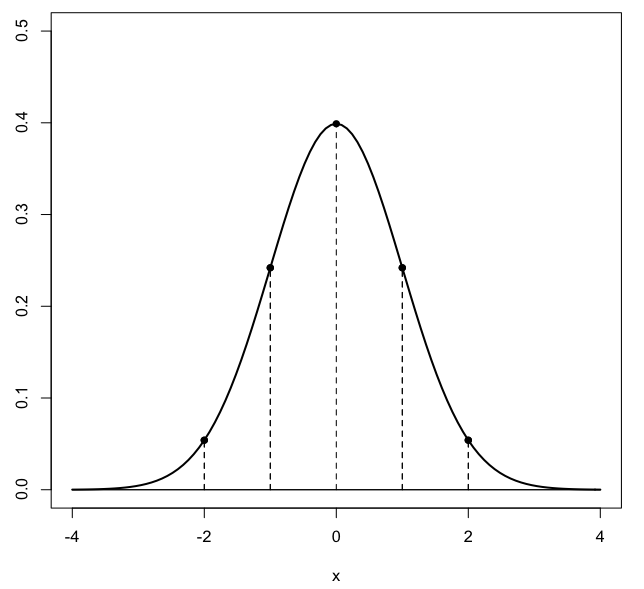
\includegraphics [scale=0.4] {gauss3.png} \end{center}
\begin{document}
\maketitle
\Large
David Joyce has proofs of the two statements of the FTC

\url{http://aleph0.clarku.edu/~ma120/FTCproof.pdf}

which we will follow here.

The two statements are often called FTC-1 and FTC-2.  Citing historical precedent, Joyce calls the second one the FTC and the first its inverse, or FTC$^{-1}$.
\subsection*{FTC}
The FTC is what we use when we evaluate definite integrals.  If $F$ is an antiderivative of $f$, then:
\[ \int_a^b f(x) \ dx = F(b) - F(a) \]
We will require that $f$ be \emph{continuous} on $[a,b]$.  Strictly speaking, this isn't necessary, but it makes the proof simpler.  For a function with a finite number of discontinuities, one can just chop up the integral into its component pieces.

For the inverse statement (FTC$^{-1}$), we require again that $f$ be continuous on $[a,b]$ and $F$ be the accumulation function defined by
\[ F(x) = \int_a^x f(t) \ dt \]
Then the theorem is that $F$ is differentiable on $[a,b]$ and its derivative is $f$.  That is
\[ F'(x) = f(x) \ \ \ \text{for } x \in [a,b] \]
This is usually written
\[ \frac{d}{dx} \ \int_a^x f(t) \ dt = f(x) \]
We have adopted the "dummy" variable $t$ to avoid confusion.
\subsection*{proof of the inverse FTC}
We start with the inverse theorem.  First of all, since $f$ is continuous, it is integrable, so we know that the integral
\[ F(x) = \int_a^x f(t) \ dt \]
actually exists.

We need to show that $F'(x) = f(x)$.  

We go back to the definition of the derivative
\[ F'(x) = \lim_{h \rightarrow 0} \ \frac{F(x+h) - F(x)}{h} \]
\[ = \lim_{h \rightarrow 0} \ \frac{1}{h} \ [ \ F(x+h) - F(x) \ ] \]
\[ = \lim_{h \rightarrow 0} \ \frac{1}{h} \ [ \ \int_a^{x+h} f(t) \ dt) - \int_a^x f(t) \ dt \ ] \]
\[ = \lim_{h \rightarrow 0} \ \frac{1}{h} \ \int_x^{x+h} f(t) \ dt \]

We will show that this limit equals $f(x)$  We will only prove the case where $h > 0$.  The other proof is similar but has minus signs in various places.

On the interval $[x, x+h]$, $f(t)$ has a minimum value $m$ and a maximum value $M$ (by the extreme value theorem).  So
\[ m \le f(t) \le M \]
for every $x \in [a,b]$,
and when we integrate each term of the inequality we get
\[ \int_x^{x+h} m \ dt \le \int_x^{x+h} f(t) \ dt \le \int_x^{x+h} M \ dt \]
Since $m$ and $M$ are constants and $\int dt = h$ between these limits:
\[ hm \le \int_x^{x+h} f(t) \ dt \le hM \]
dividing through by $h$
\[ m \le \frac{1}{h} \int_x^{x+h} f(t) \ dt \le M \]
Now, as $h \rightarrow 0$, all values of $f$ on the interval $[x,x+h]$ approach the same value, and in particular, $m \rightarrow f(x)$ and $M \rightarrow f(x)$.  Being squeezed between them
\[ \lim_{h \rightarrow 0} \ \frac{1}{h} \int_x^{x+h} f(t) = f(x) \]
$\square$

\subsection*{proof of the FTC}
Let 
\[ G(x) = \int_a^x F'(t) \ dt \]
Take derivatives on both sides
\[ G'(x) = \frac{d}{dx} \ \int_a^x F'(t) \ dt \]
so
\[ G'(x) = F'(x) \]
by the theorem we just proved.

Therefore $G(x)$ and $F(x)$ differ at most by a constant
\[ G(x) = F(x) + C \]
for $x \in [a,b]$.

In particular, at $x = a$ we have
\[ G(a) = F(a) + C \]
but
\[ G(a) = \int_a^a F'(t) \ dt = 0 \]
Hence
\[ F(a) = - C \]
At $x = b$ we have
\[ G(b) = F(b) + C \]
but $C = - F(a)$
so
\[ G(b) = F(b) - F(a) \]
By the original definition of $G$
\[ G(b) = \int_a^b F'(t) \ dt \]
Hence
\[ \int_a^b F'(t) \ dt = F(b) - F(a) \]
$\square$
\end{document}  